\documentclass[11pt]{article}
\usepackage{verbatim, amsmath, amssymb, hyperref,enumerate,multicol}
\pagestyle{empty}
\voffset=-.5in
\textheight=8.75in
\textwidth=6in
\hoffset=-.35in

\newcommand{\ls}{\vspace{.1in}}
\newcommand{\ds}{\displaystyle}


\usepackage{fancyhdr}
\pagestyle{fancy}
\lhead{Math Foundations}
\rhead{Written HW 5}
\cfoot{\thepage}
\renewcommand{\headrulewidth}{0.4pt}
\renewcommand{\footrulewidth}{0.4pt}
\usepackage{tikz}

\begin{document}

\centerline{\bf Written Homework 5}


\centerline{Name(s): Elliot Marshall}

\begin{itemize}
\begin{comment}
\item[4.3.10.] The sequence in Exercise~4.3.9 is an example of an \emph{arithmetic sequence}. An arithmetic sequence is defined as follows:

Let $c$ and $d$ be real numbers. Define the sequence $a_1,a_2,\dots, a_n,\dots$ by $a_1=c$ and for each $n\in \mathbb{N}$, $a_{n+1}=a_n+d$.
\begin{enumerate}[(a)]
\item Determine formulas for $a_3$ through $a_8$.
\item Make a conjecture for a formula for $a_n$ for each $n\in\mathbb{N}$.
\item Prove that your conjecture in the previous part is true.
\end{enumerate}

\hrulefill\end{comment}

\item[5.1.9.] Let $P$, $Q$, $R$, and $S$ be subsets of a universal set $U$. Assume that $(P-Q)\subseteq(R\cap S)$.
\begin{enumerate}[(a)]
\item Complete the following sentence:
\begin{quote}
For each $x\in U$, if $x\in(P-Q)$, then \dots
\end{quote}
\begin{quote}
For each $x\in U$, if $x\in(P-Q)$, then $x\in R$ and $x\in S$.
\end{quote}

\item Write a useful negation of the statement in part (a). 
\begin{quote}
For each $x\in U$, if $x\in(P-Q)$ then $x\not\in R$ or $x\not\in S$.
\end{quote}

\item Write the contrapositive of the statement in part (a).
\begin{quote}
For each $x\in U$, if $x\not\in R$ or $x\not\in S$ then $x\not\in(P-Q)$.
\end{quote}
\end{enumerate}


\hrulefill

\item[5.2.11.] Let $A$, $B$, $C$, and $D$ be subsets of some universal set $U$. Are the following propositions true or false? Justify your conclusions.
\begin{enumerate}[(a)]
\item If $A\subseteq B$ and $C\subseteq D$ and $A$ and $C$ are disjoint, then $B$ and $D$ are disjoint.
\begin{quote}
    False. It does not follow that two disjoint subsets necessitates that their supersets are disjoint.\\
    For example, let $A=\{1,3\}$, $B=\{1,3,5\}$, $C=\{2,4\}$, and $D=\{2,4,5\}$. Then $A\subseteq B$, $C\subseteq D$, $A$ and $C$ are disjoint, 
    while $B$ and $D$ are not disjoint as $5\in B$ and $5\in D$.
\end{quote}
\item If $A\subseteq B$ and $C\subseteq D$ and $B$ and $D$ are disjoint, then $A$ and $C$ are disjoint.
\begin{quote}
    True. If two sets are truly disjoint, then their respective subsets must by defination share no common values, thus making those subsets disjoint 
    as well. Furthermore, $A$ and $D$ along with $B$ and $C$ are each disjoint.
\end{quote}
\end{enumerate}

\hrulefill

\item[5.3.8] Let $A$, $B$, and $C$ be subsets of some universal set $U$.
\begin{enumerate}[(a)]
\item Draw two general Venn diagrams for the sets $A$, $B$, and $C$. On one, shade the region that represents $A-(B-C)$, and on the other, shade 
the region that represents $(A-B)\cup(A-C^c)$. Based on the Venn diagrams, make a conjecture about the relationship between the sets $A-(B-C)$ 
and $(A-B)\cup(A-C^c)$. (Are the two sets equal? If not, is one of the sets a subset of the other set?)\\ \\
\begin{center}
    \pagebreak
    Venn Diagram 1: $A-(B-C)$\\
    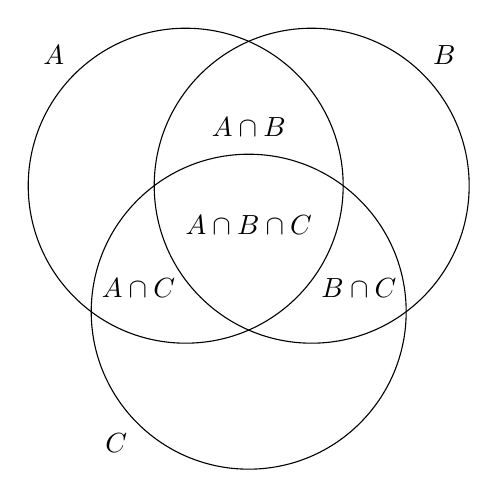
\begin{tikzpicture}
 
        % Set A
        \node [draw,
            circle,
            minimum size =4cm,
            label={135:$A$}] (A) at (-0.8,0){};
         
        % Set B
        \node [draw,
            circle,
            minimum size =4cm,
            label={45:$B$}] (B) at (0.8,0){};

        \node [draw,
            circle,
            minimum size =4cm,
            label={225:$C$}] (C) at (0,-1.6){};
         
        % Set intersection labels
        \node at (0,0.75) {$A\cap B$};
        \node at (-1.4,-1.3) {$A\cap C$};
        \node at (1.4,-1.3) {$B\cap C$};
        \node at (0.0,-0.5) {$A\cap B\cap C$};
         
        \end{tikzpicture}

        Venn Diagram 2: $(A-B)\cup(A-C^c)$ \\
        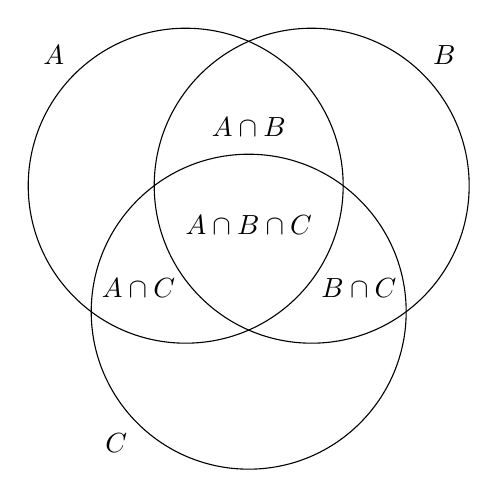
\begin{tikzpicture}
     
            % Set A
            \node [draw,
                circle,
                minimum size =4cm,
                label={135:$A$}] (A) at (-0.8,0){};
             
            % Set B
            \node [draw,
                circle,
                minimum size =4cm,
                label={45:$B$}] (B) at (0.8,0){};
    
            \node [draw,
                circle,
                minimum size =4cm,
                label={225:$C$}] (C) at (0,-1.6){};
             
            % Set intersection labels
            \node at (0,0.75) {$A\cap B$};
            \node at (-1.4,-1.3) {$A\cap C$};
            \node at (1.4,-1.3) {$B\cap C$};
            \node at (0.0,-0.5) {$A\cap B\cap C$};
             
            \end{tikzpicture}
\end{center}
Conjecture: $A-(B-C)=(A-B)\cup (A-C^c)$
\item Prove the conjecture from part (a).
\begin{quote}
    Proof: Let $x\in A-(B-C)$. Then $x\in A$ and $x\not\in (B-C)$ \\
    $\rightarrow$ $x\in A$ and $x\in C$ while $x\not\in B$. \\
    $\rightarrow$ $(x\in A$ and $x\not\in B)$ or $(x\in A$ and $x\in C)$\\
    $\rightarrow$ $x\in(A-B)$ or $(x\in A$ and $x\not\in C^c)$ \\
    $\rightarrow$ $x\in(A-B)\cup x\in(A-C^c)$ \\
    $\rightarrow$ $x\in (A-B)\cup(A-C^c)$. QED
\end{quote}
\end{enumerate}

\end{itemize}



\end{document}